\chapter{Generering af signal}
I dette kapitel genereres et signal $s(n)$, som skal samples til $s[n]$. I projektbeskrivelsen er følgende krav til signalet opgivet:
\begin{itemize}
\setlength\itemsep{0em}
\item Signalet skal bestå af en sum af tre individuelle sinus-komponenter.
\item De tre frekvenser af komponenterne skal findes ved $\omega_1=\pi/3$, $\omega_2=\pi/2$ og $\omega_3=3\pi/4$, alle i $\text{rad}/\text{s}$.
\item Komponenterne skal have indbyrdes fasedrej på $\varphi=2\pi/3$ rad.
\item Komponenterne skal have ens amplitude.
\end{itemize}
På baggrund af ovenstående krav er følgende signal opstillet:
\begin{align}
s(n)&=\sin\left(\omega_1n\right)+\sin\left(\varphi+\omega_2n\right)+\sin\left(2\varphi+\omega_3n\right)\\
&=\sin\left(\frac{\pi}{3}n\right)+\sin\left(\frac{2\pi}{3}+\frac{\pi}{2}n\right)+\sin\left(\frac{4\pi}{3}+\frac{3\pi}{4}n\right)\label{eq:signal}
\end{align}
I figur \ref{fig:signal} ses signalet.
\begin{figure}[H]
\centering
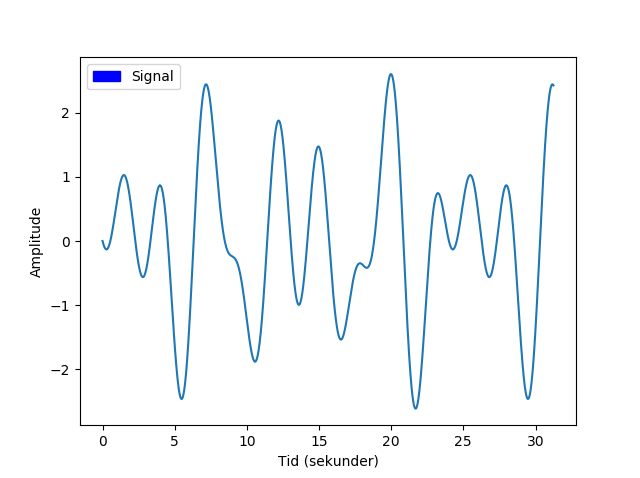
\includegraphics[width=0.7\textwidth]{figures/signal.png}
\caption{Plot af signal i lidt over en periode.}
\label{fig:signal}
\end{figure}
\section{Sampling}
For at kunne simulere signalet \eqref{eq:signal} i Python og efterfølgende lave frekvensanalyse og filtrering af det, kræves det at signalet samples. 
For at undgå spejling som følge af for langsom samplingsfrekvens $f_s$ bruges Nyquist-Shannos samplingsteorem, som siger, at et signal kan fuldstændigt bestemmes ud fra dets samples, hvis det samples med en samplingsfrekvens $f_s$ således, at
\begin{align}
f_s>2B,
\end{align}
hvor $B$ er den højeste frekvens optrædende i signalet. Altså bestemmes nu $B$ ved at bestemme den højeste frekvens optrædende i signalet$^[$\footnote{Det antages, at $s(n)$ er båndbegrænset.}$^]$:
\begin{align*}
f_1&=\frac{\omega_1}{2\pi}=\frac{1}{6}\text{ Hz}\\
f_2&=\frac{\omega_2}{2\pi}=\frac{1}{4}\text{ Hz}\\
f_3&=\frac{\omega_3}{2\pi}=\frac{3}{8}\text{ Hz}
\end{align*}
Det ses, at $f_3=\frac{3}{8}$ Hz er den højeste frekvens i signalet. Altså haves $B=\frac{3}{8}$ Hz og Nyquistraten $2B=\frac{3}{4}$ Hz. Fra dette konkluderes, at en samplingsfrekvens, der opfylder
\begin{align}
f_s>\frac{3}{4}\text{ Hz}
\end{align}
vil medføre, at der ikke sker spejling, når $s(n)$ samples. I figur \ref{fig:s_sampled} ses $s(n)$ samplet ved $f_s=1$ Hz.\todo{Den her frekvens skal nok tilpasses, således filtreringen går nemmere.}
\begin{figure}[H]
\centering
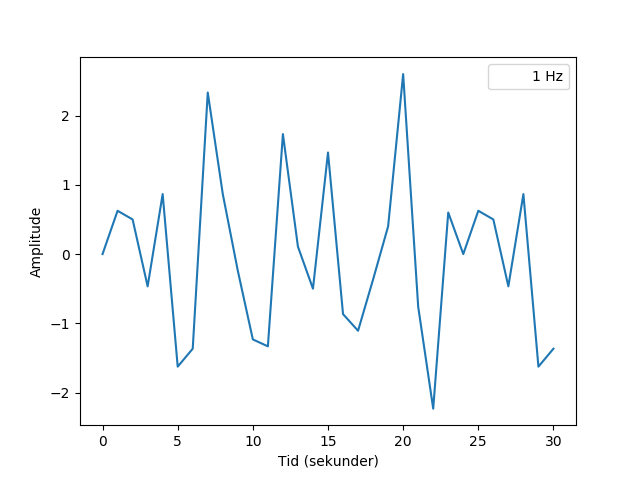
\includegraphics[width=0.7\textwidth]{figures/signal_1hz}
\caption{Signal samplet ved 1 Hz.}
\label{fig:s_sampled}
\end{figure}
Med $s[n]$, som fuldstændigt bestemmer $s(n)$, fortsættes nu til frekvensanalysen.